\documentclass[aspectratio=169,11pt]{beamer}

\usepackage{graphicx,amsmath,amssymb,tikz,psfrag,verbatim}
\usepackage{tikz}
\usepackage{fancyvrb}
\usepackage{kotex}
%\usepackage{mcode}
\usepackage{listings}
\usepackage{xcolor}
\usepackage{animate}
\usetikzlibrary{shapes.geometric}

\input lecturedefs.tex
\input listing_defs.tex

\graphicspath{{img/}}

%% formatting

\mode<presentation>
{
\usetheme{default}
}
\setbeamertemplate{navigation symbols}{}
\usecolortheme[rgb={0.13,0.28,0.59}]{structure}
\setbeamertemplate{itemize subitem}{--}
\newcommand\footlineon{
\setbeamertemplate{footline} {
\begin{beamercolorbox}[ht=2.5ex,dp=1.125ex,leftskip=.8cm,rightskip=.6cm]{structure}
%\footnotesize \insertsection
\hfill
{\insertframenumber}
\end{beamercolorbox}
\vskip 0.45cm
}
}
\footlineon

\AtBeginSection[] 
{ 
\begin{frame}<beamer> 
\frametitle{Outline} 
\tableofcontents[currentsection,currentsubsection] 
\end{frame} 
} 

%% begin presentation

\title{\large \bfseries Convex-Concave Procedure}
\author{Stephen Boyd \and Max Schaller \and Daniel Cederberg}
%\date{March XXX 2025}


\begin{document}
\frame{
\thispagestyle{empty}
\titlepage
}

\begin{frame}{Overview}
the \textbf{convex-concave procedure} (CCP)
\BIT
\item is a heuristic method for solving a specific type of 
nonconvex problem
\item involves solving a (typically small) sequence
of convex problems
\item leverages expressiveness and reliability of convex optimization
\item is a good street-fighting trick to know about
\EIT
\end{frame}


\section{Difference of convex functions}

\begin{frame}{Difference of convex functions}

\BIT
\item a \textbf{difference of convex} (DC) function $h:\reals^n \to \reals$ 
has the form 
\[
h(x)=f(x)-g(x)
\]
with $f$ and $g$ convex
\item any function with continuous second derivative
has this form, but most useful when we have explicit expressions 
for $f$ and $g$
\EIT
\end{frame}


\begin{frame}{Examples}
\begin{columns}
\begin{column}{0.5\textwidth}
\centering
$f(x) = x^4 + 0.2 x, \quad g(x) = x^2$ \\
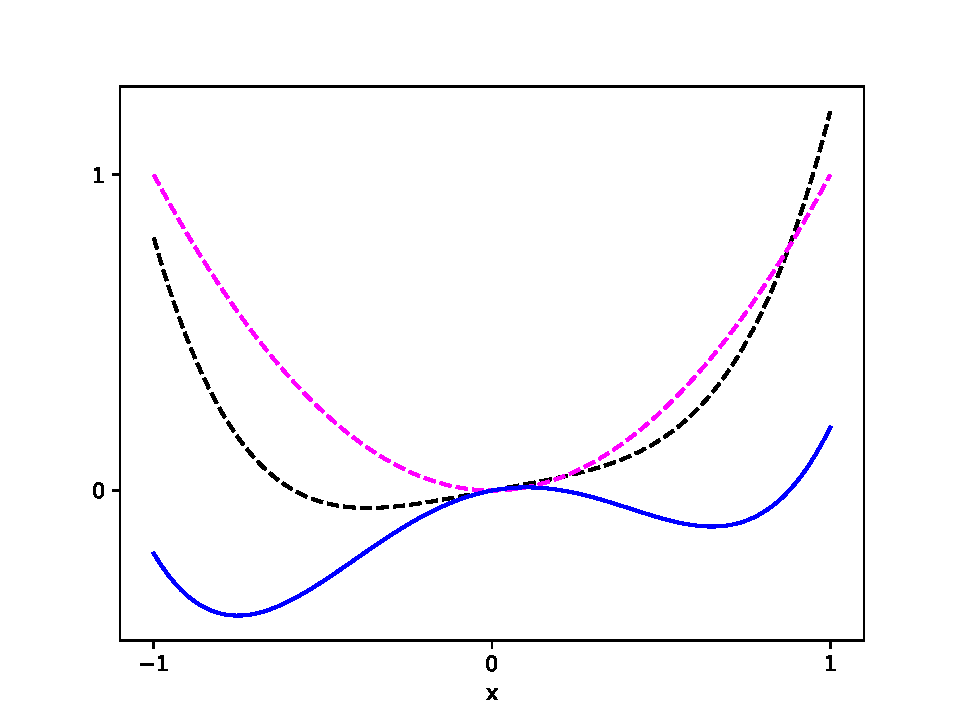
\includegraphics[width=\textwidth]{DC1.pdf}
\end{column}
\begin{column}{0.5\textwidth}
\centering
$f(x) = (x^3)_+, \quad g(x) = (x^3)_-$ \\
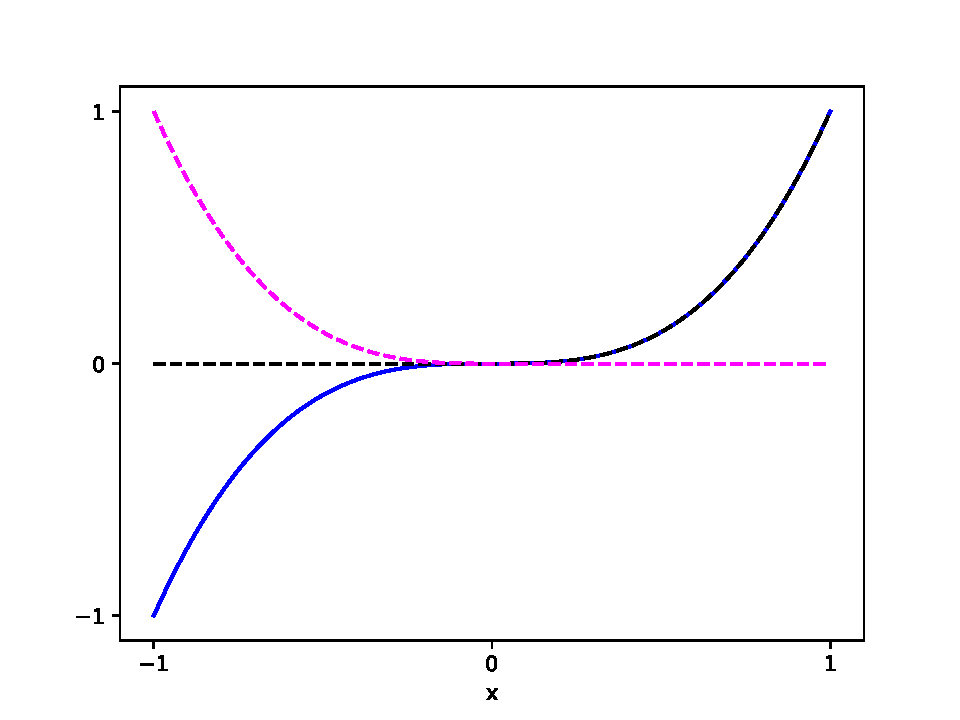
\includegraphics[width=\textwidth]{DC2.pdf}
\end{column}
\end{columns}
\vfill\centering
$f(x)$ in black,
$g(x)$ in \textcolor{magenta}{magenta},
$h(x) = f(x) - g(x)$ in \textcolor{blue}{blue}
\end{frame}

\begin{frame}{Quadratic function as DC}
\BIT
\item (nonconvex) quadratic function $h(x)= (1/2)x^TPx+q^Tx + r$, $P\in \symm^n$
\item decompose $P$ into its PSD and NSD parts $P=P_\text{psd} - P_\text{nsd}$, 
$P_\text{psd},P_\text{nsd}\succeq 0$
\BIT
\item $P = Q\Lambda Q^T$ is eigenvalue decomposition
\item $P_\text{psd} = Q\Lambda_+ Q^T$, with 
$\Lambda_+ = \max\{0,\Lambda\}$ (elementwise)
\item $P_\text{nsd} = Q\Lambda_- Q^T$, with 
$\Lambda_- = \max\{0,-\Lambda\}$ (elementwise)
\EIT
\item express $h$ in DC form as $h=f-g$ with
\[
f(x)= (1/2)x^TP_\text{psd}x+q^Tx + r, \qquad g(x)=(1/2)x^TP_\text{nsd}x 
\]
\EIT
\end{frame}

\begin{frame}{A simple majorizer for a DC function}
\BIT
\item if (convex) $g$ is differentiable, then for all $x$
\[
\hat g(x;z) = g(z)+ \nabla g(z)^T (x-z) \leq g(x)
\]
(for nondifferentible $g$, replace $\nabla g(x)$ with any subgradient)
\item for DC function $h=f-g$, define
\[
\hat h(x;z)= f(x)-\hat g(x;z)
\]
\item $\hat h$ is convex (in $x$) and satisfies
$\hat h(x;z) \geq h(x)$ for all $x$,
$\hat h(z;z) = h(z)$
\item \ie,
$\hat h(x;z)$ is a \textbf{majorizer} of $g$, tight at $z$
\EIT
\end{frame}

\begin{frame}{Examples}
\begin{columns}
\begin{column}{0.5\textwidth}
\centering
$h(x) = x^4 + 0.2 x - x^2$, \\ majorized at $z=0.3$ \\
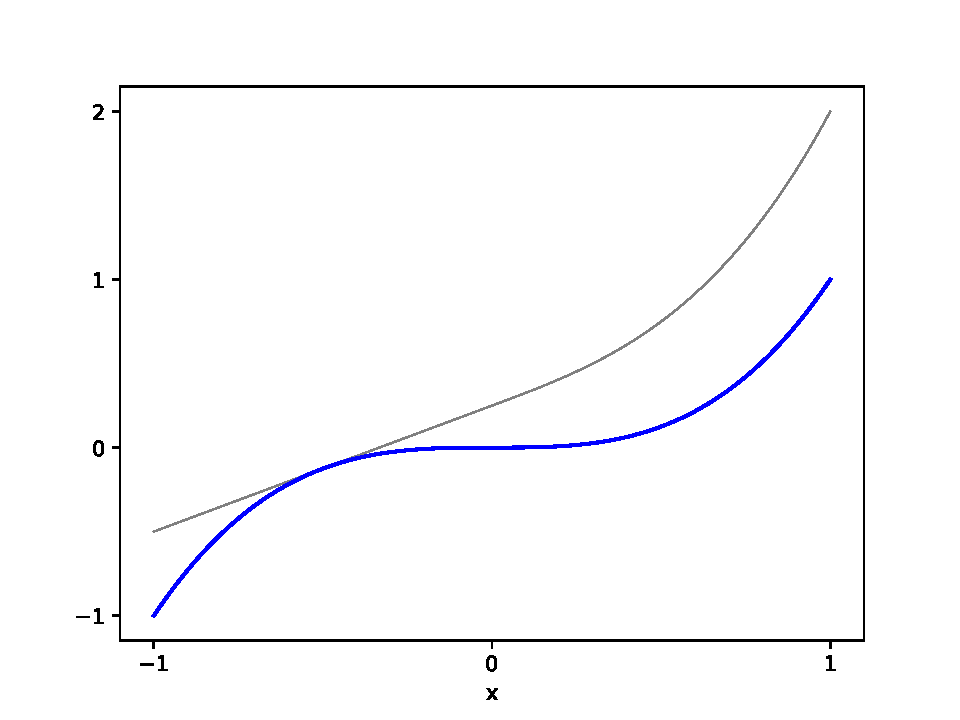
\includegraphics[width=\textwidth]{DC1_majorized.pdf}
\end{column}
\begin{column}{0.5\textwidth}
\centering
$h(x) = (x^3)_+ - (x^3)_- = x^3$, \\ majorized at $z=-0.5$ \\
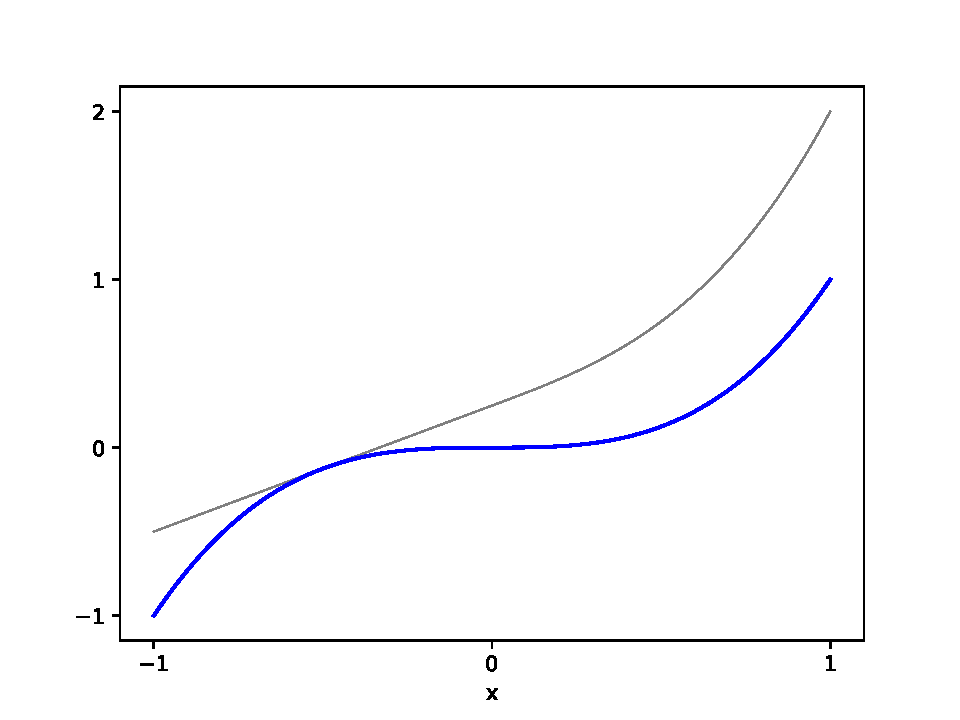
\includegraphics[width=\textwidth]{DC2_majorized.pdf}
\end{column}
\end{columns}
\vfill\centering
$h(x)$ in \textcolor{blue}{blue},
$\hat h(x; z)$ in \textcolor{gray}{gray}
\end{frame}

\section{Convex-concave procedure}
\begin{frame}{Minimizing a DC function}
\BIT
\item (unconstrained) \textbf{DC problem}: minimize DC function $h(x)=f(x)-g(x)$
\item convex constraints can be handled as indicator functions added to $f$
\item \textbf{convex-concave procedure} (CCP): iterate
\[
x^{k+1} = \argmin_x \hat h(x;x^k) =
\argmin_x \left( f(x) - \hat g(x;x^k)\right)
\]
\item $x^{k+1}$ can be found via convex optimization
\item CCP has no parameters, no line search / trust penalty, \ldots
%\item convex constraints can be handled as indicator function added to $f$
\EIT
\end{frame}

\begin{frame}{Properties of CCP}
\BIT
\item CCP is a \textbf{descent method}:
\[
h(x^{k+1}) \leq \hat h(x^{k+1};x^k) \leq \hat h(x^k;x^k)=h(x^k)
\]
\item $h(x^k)$ converges, but not necessarily to $h^\star = \inf_x h(x)$
\item ultimate value $\lim_{k\to \infty} h(x^k)$ depends on initial point $x^0$
\item standard trick: run CCP for multiple initial points; take best ultimate point found
\EIT
\end{frame}

%\begin{frame}{CCP for minimizing a DC function} 
%\BIT
%\item is a sophisticated heuristic
%\item solves a convex optimization problem in each iteration
%\item can converge to different points depending on initial point
%\item is a special case of \textbf{majorization-minimization} (MM) algorithm
%\EIT
%\end{frame}

\begin{frame}{Example}
\centering
$f(x) = x^4 + 0.2 x$, $g(x) = x^2$, initialized at $x^0 = -0.2$ \\
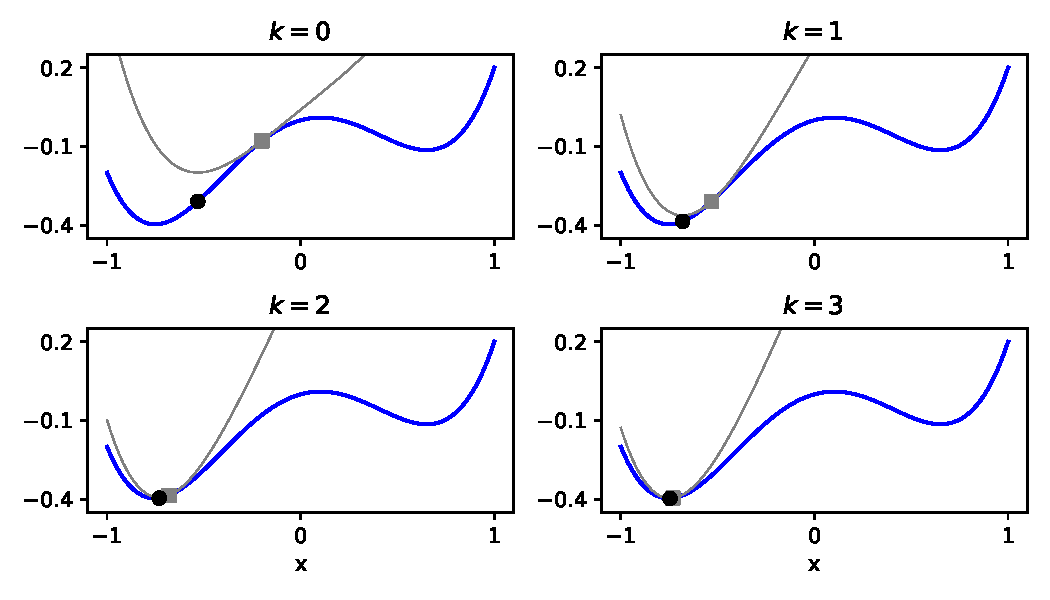
\includegraphics[width=0.7\textwidth]{DC1_iterations_left.pdf} \\
$h(x)$ in \textcolor{blue}{blue},
$\hat h(x;x^k)$ in \textcolor{gray}{gray}, \\
$(x^k, h(x^k))$ as squares,
$(x^{k+1}, h(x^{k+1}))$ as circles
\end{frame}

\begin{frame}{Example}
\centering
$f(x) = x^4 + 0.2 x$, $g(x) = x^2$, initialized at $x^0 = 0.2$ \\
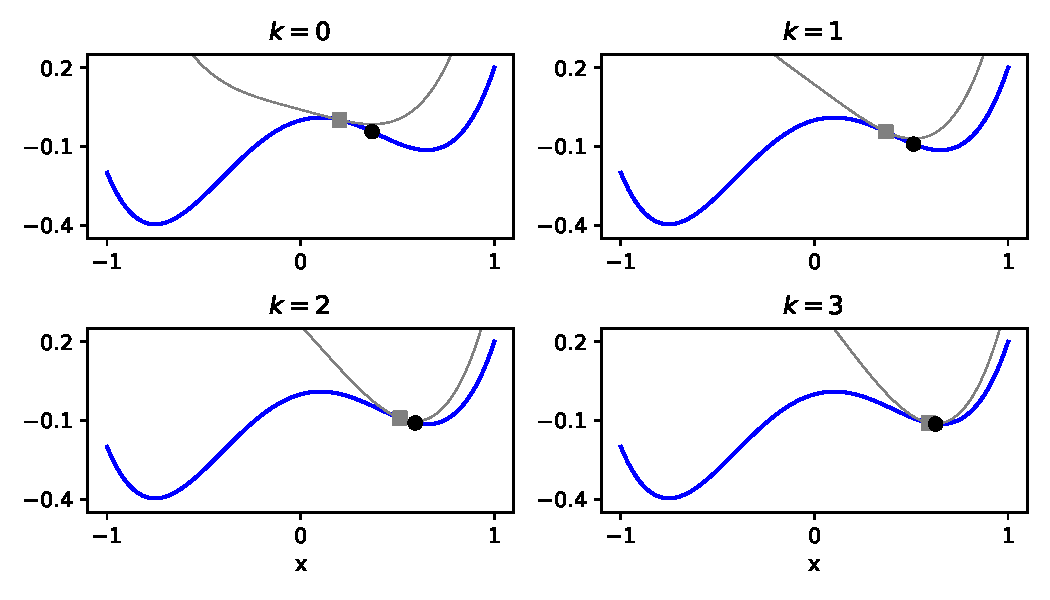
\includegraphics[width=0.7\textwidth]{DC1_iterations_right.pdf} \\
$h(x)$ in \textcolor{blue}{blue},
$\hat h(x;x^k)$ in \textcolor{gray}{gray}, \\
$(x^k, h(x^k))$ as squares,
$(x^{k+1}, h(x^{k+1}))$ as circles
\end{frame}

\begin{frame}{SAT problem}
\BIT
\item SAT problem: find $x_i \in \{0,1\}$ with $Ax \preceq b$
\item includes 3-SAT; NP-hard
\item encode Boolean constraint using $x_i \in \{0,1\} ~\Longleftrightarrow~
x_i^2-x_i = 0$
\item SAT problem equivalent to minimizing DC function $h=f-g$ with
\[
f(x) = \left\{ \begin{array}{ll} 0 & Ax \preceq b,~0 \preceq x \preceq \ones\\
\infty & \mbox{otherwise}
\end{array}\right. \qquad 
g(x) = \sum_{i=1}^n (x_i^2-x_i)
\]
since $h(x) \geq 0$ for all $x$ and
\[
h(x) = 0 \quad \Longleftrightarrow \quad Ax \preceq b,~~x_i \in \{0,1\},
~i=1, \ldots, n
\]
\EIT
\end{frame}

\begin{frame}{SAT problem via CCP}
\BIT
\item CCP: $x^{k+1}$ is a solution of LP
\[
\begin{array}{ll}
\mbox{minimize} & (\ones - 2 x^k) ^T x \\
\mbox{subject to} & Ax \preceq b, \quad 0 \preceq x \preceq \ones
\end{array}
\]
\item \textbf{example:} 
find $x \in \{0, 1\}^4$ that satisfies predicate
\[
(x_1 \lor x_2 \lor \neg x_3) \land (\neg x_1 \lor \neg x_2 \lor x_4)
\land (\neg x_2 \lor x_3 \lor \neg x_4)
\]
(a feasible 3-SAT instance with $n=4$ variables and $3$ clauses)
\item can be represented as
\[
A = \left[\begin{array}{rrrr}
-1 & -1 & 1 & 0 \\
1 & 1 & 0 & -1 \\
0 & 1 & -1 & 1 \\
\end{array}\right],
\quad b = \left[\begin{array}{r}
0 \\ 1 \\ 1
\end{array}\right]
\]
\EIT
\end{frame}

\begin{frame}[fragile]{SAT problem via CCP}
\begin{columns}
\begin{column}{0.6\textwidth}
\begin{verbatim}
n = 4
x = Variable(n)
xk = Parameter(n)

obj = Minimize((ones(n) - 2 * xk) @ x)
constr = [A @ x <= b, 0 <= x, x <= 1]
prob = Problem(obj, constr)

xk.value = ones(n) / 2
for _ in range(3):
    prob.solve()
    xk.value = x.value
\end{verbatim}
\end{column}
\begin{column}{0.4\textwidth}
\hspace{60pt} $x^k$
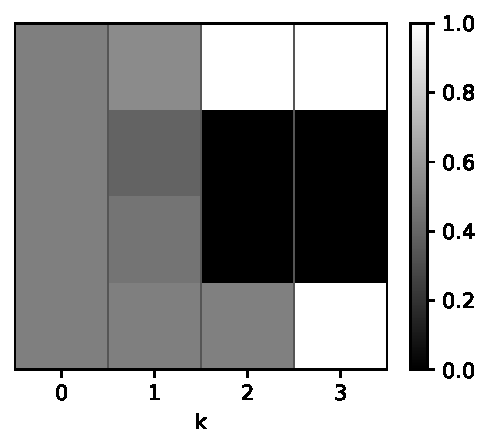
\includegraphics[width=\textwidth]{sat_small.pdf}
\end{column}
\end{columns}
\end{frame}

\begin{frame}[fragile]{SAT problem via CCP}
larger example, (feasible) 3-SAT instance with $n=40$, $120$ clauses
\vfill
\begin{columns}
\begin{column}{0.6\textwidth}
\centering
$h(x^k)$ \\
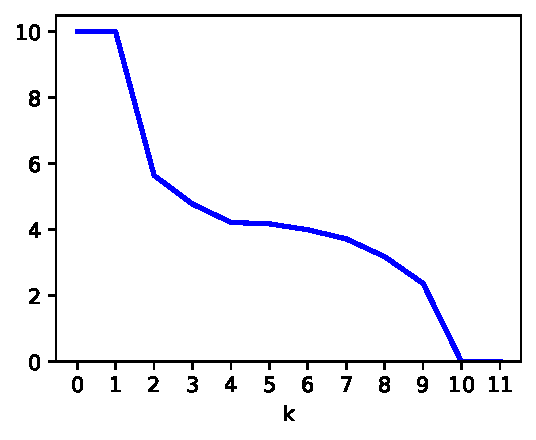
\includegraphics[width=0.7\textwidth]{sat_large_value.pdf}
\end{column}
\begin{column}{0.4\textwidth}
\hspace{60pt} $x^k$\\
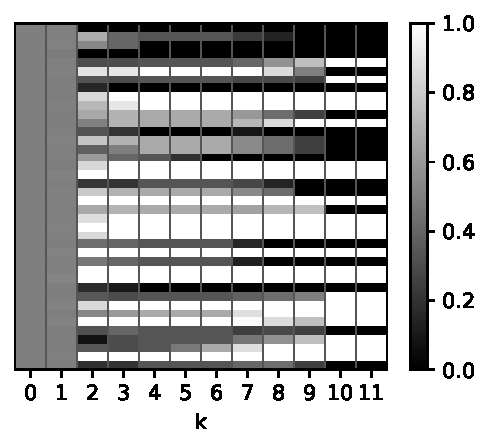
\includegraphics[width=\textwidth]{sat_large.pdf}
\end{column}
\end{columns}

finds feasible point for 19\% of random initializations
\end{frame}

\begin{frame}{Constrained DC problem}
\BIT
\item \textbf{DC problem} with DC inequality constraints has form
\[
\begin{array}{ll}
\mbox{minimize} & f_0(x) - g_0(x) \\
\mbox{subject to} & f_i(x) - g_i(x) \leq 0, \quad i = 1, \ldots, m
\end{array}
\]
$f_i$ and $g_i$ are convex
\item CCP algorithm: $x^{k+1}$ is solution of convex problem
\[
\begin{array}{ll}
\mbox{minimize} & f_0(x) - \hat g_0(x;x^k)\\
\mbox{subject to} & f_i(x) - \hat g_i(x;x^k) \leq 0, \quad i = 1, \ldots, m
\end{array}
\]
\item in words: linearize concave parts; solve; repeat
\item if $x^k$ is feasible, then so is $x^{k+1}$,
and $h(x^{k+1}) \leq h(x^k)$
\item CCP is a feasible descent method
\EIT
\end{frame}

\begin{frame}{Convex restrictions}
\BIT
\item if
$\hat h_i(x;x^k) = f_i(x) - \hat g_i(x;x^k)\leq 0$, then
$h_i(x) \leq \hat h_i(x;x^k) \leq 0$
\item so convexified constraint is a \textbf{convex restriction} of original 
constraint
\item \textbf{example}: $f(x) = 0$, $g(x) = \|x\|_2 - 1$, 
$x^k =(3, 1)$ (left) and $x^k=(1, 2)$ (right)
\EIT
\centering
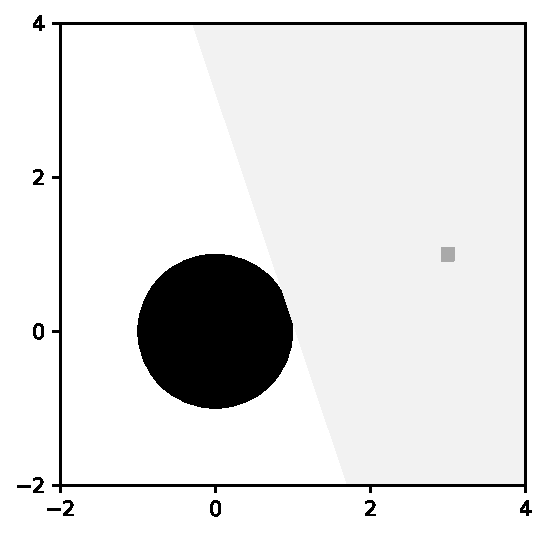
\includegraphics[width=0.25\textwidth]{convex_restriction_31.pdf}
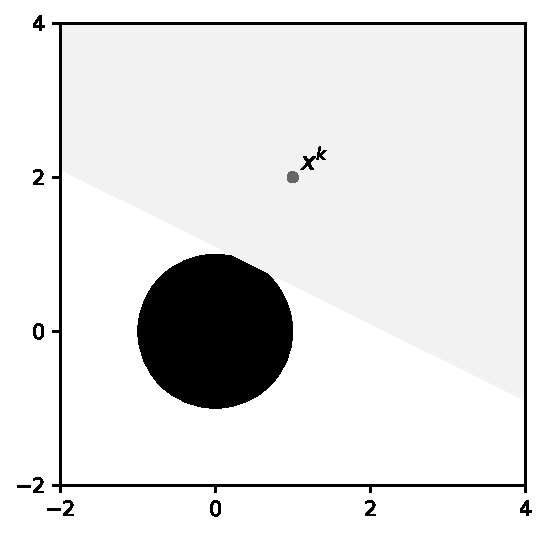
\includegraphics[width=0.25\textwidth]{convex_restriction_12.pdf} \\
$h(x)\leq 0$ in white,
$\hat h(x;x^k)\leq 0$ in gray ($x^k$ as gray dot)
\end{frame}

\begin{frame}{Convex restrictions}
\BIT
\item \textbf{example}: CCP for simple problem
\[
\begin{array}{ll}
\mbox{minimize} & \|x - c\|_2 \\
\mbox{subject to} & \|x\|_2 \geq 1
\end{array}
\]
with variable $x \in \reals^2$, data $c$ with $\|c\|_2 < 1$, $c \neq 0$
\item \ie, find closest point to $c$ that is \textbf{outside} unit ball
\item solution is $x^\star = c/\|c\|_2$
\item consider $c = (-0.4, 0.6)$ and $x^0 = (2.5, 1)$
\EIT
\end{frame}

\begin{frame}{CCP iterations}
\centering
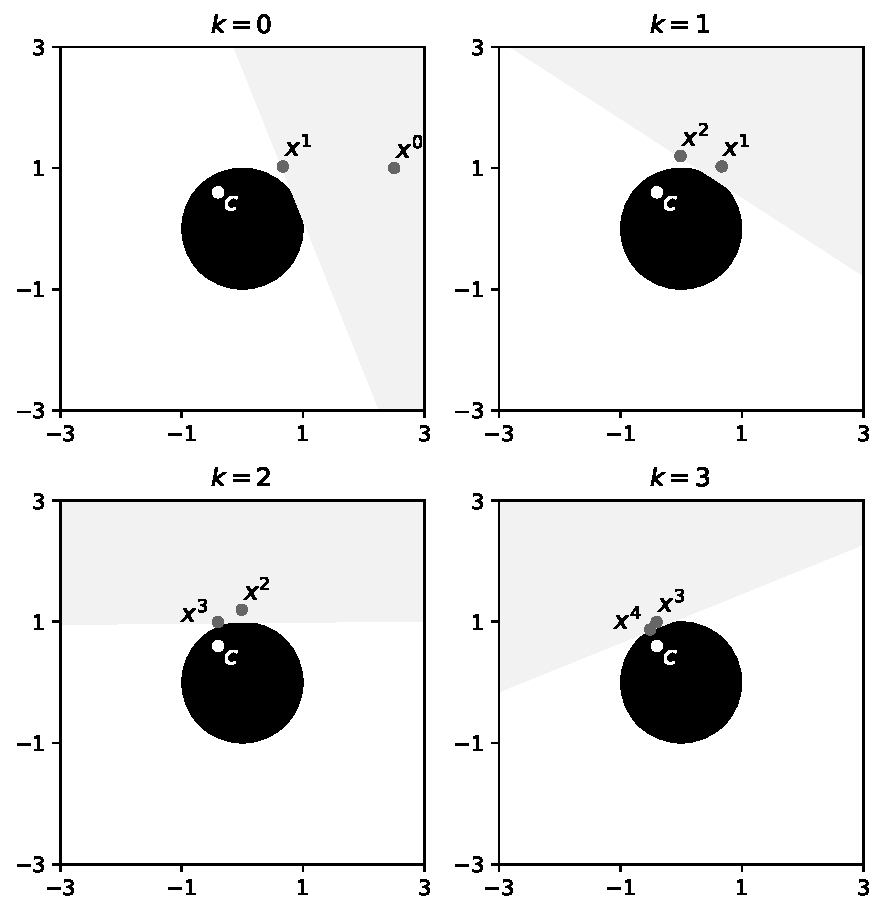
\includegraphics[width=0.5\textwidth]{convex_restriction_iterations.pdf} \\
$x^k$ as a square, $x^{k+1}$ as a circle, $c$ as a cross
\end{frame}

\begin{frame}{CCP iterations}
\centering
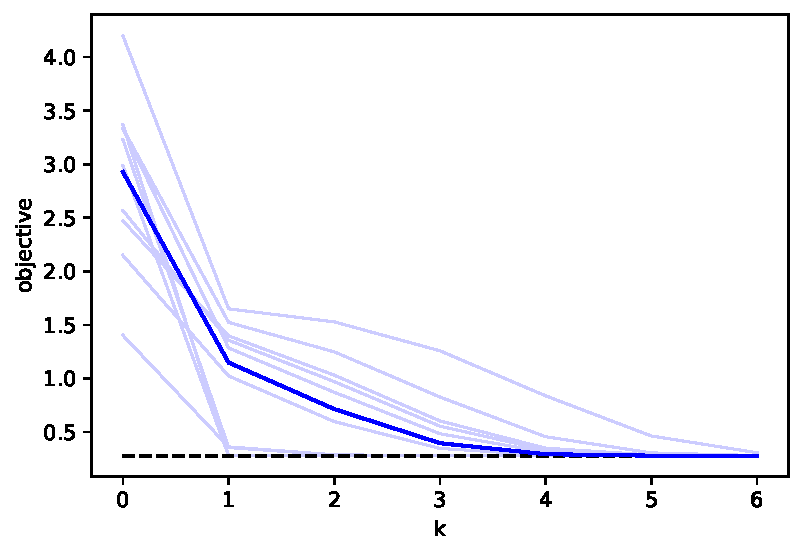
\includegraphics[width=0.6\textwidth]{convex_restriction_iterations_value.pdf} \\
$\|x^k - c\|_2$ in \textcolor{blue}{blue},
$\|x^\star - c\|_2 = 1-\|c\|_2$ as dashed black line
\end{frame}

\begin{frame}{DC equality constraints}
\BIT
\item linear equality constraints can just be added as indicator 
function to $f$
\item DC equality constraints of the form $p_i(x) = q_i(x)$,
with $p_i$ and $q_i$ convex,
can be expressed as the pair of DC inequalities
\[
p_i(x) - q_i(x) \leq 0, \qquad q_i(x) - p_i(x) \leq 0
\]
\EIT
\end{frame}

\begin{frame}{Ensuring feasibility of convex subproblems}
\BIT
\item convex subproblems can be infeasible,
even if original problem is feasible
\item introduce \textbf{slack variable} $s_i \geq 0$ for constraint $i$
\item \textbf{penalty CCP} algorithm:
$x^{k+1}$ is solution of convex problem
\[
\begin{array}{ll}
\mbox{minimize} & f_0(x) - \hat g_0(x;x^k) + \tau_k \sum_{i=1}^m s_i\\
\mbox{subject to} & f_i(x) - \hat g_i(x;x^k) \leq s_i, \quad i = 1, \ldots, m\\
& s_i \geq 0, \quad i = 1, \ldots, m
\end{array}
\]
where $\tau_k > 0$ is increased between iterations
\EIT
\end{frame}

\begin{frame}{Disciplined convex-concave programming (DCCP)}
\BIT
\item \textbf{disciplined convex-concave program} (DCCP) has form
\[
\begin{array}{ll}
\mbox{minimize/maximize} & o(x) \\
\mbox{subject to} &l_i(x) \sim r_i(x), \quad i = 1, \ldots, m,
\end{array}
\]
\item $o,l_i,r_i$ are DCP convex or concave expressions
\item $\sim$ can be $\leq$, $\geq$, or $=$
\item to minimize DC objective $f_0-g_0$
\BIT
\item introduce epigraph variable $t$ and DCCP constraint $f_0(x)-g_0(x) \leq t$
\item minimize $t$
\EIT
\item implemented in DCCP package
\EIT
\end{frame}

\begin{frame}[fragile]{Disciplined convex-concave programming (DCCP)}
\begin{columns}
\begin{column}{0.5\textwidth}
\BIT
\item \textbf{example (revisited)}:
\[
\begin{array}{ll}
\mbox{minimize} & \|x - c\|_2 \\
\mbox{subject to} & \|x\|_2 \geq 1
\end{array}
\]
with variable $x \in \reals^2$, data $c$
\EIT
\end{column}
\begin{column}{0.5\textwidth}
\begin{verbatim}
x = Variable(2)
obj = Minimize(norm(x - c))
constr = [norm(x) >= 1]
prob = Problem(obj, constr)

x.value = [2.5, 1]
prob.solve(method='dccp')
print(x.value)
\end{verbatim}
\end{column}
\end{columns}
\end{frame}

\section{Examples}

\begin{frame}{Path planning with obstacles}
\BIT
\item find shortest path connecting points $a$ and $b$ in $\reals^d$,
avoiding $m$ disks
\item disk $j$ has center $c_j$, radius $r_j$
\item discretize path as points $x_0, \ldots, x_n$ and solve
\[
\begin{array}{ll}
\mbox{minimize} & L\\
\mbox{subject to} &x_0 = a, \quad x_n = b\\
& \|x_i - x_{i-1}\|_2 \leq L/n, \quad i = 1, \ldots, n\\
& \|x_i - c_j\|_2 \geq r_j, \quad i = 1, \ldots, n, \quad j = 1, \ldots, m
\end{array}
\]
with variables $L$ and $x$
\item useful initialization: straight line connecting $a$ and $b$
\EIT
\end{frame}

\begin{frame}[fragile]{Path planning with obstacles}
\begin{verbatim}
L = Variable()
x = Variable((n+1, d))
L.value, x.value = ...  # initialize to straight line

constr = [x[0] == a, x[n] == b]
for i in range(1, n+1):
    constr += [norm(x[i] - x[i-1]) <= L/n]
for j in range(m):
    constr += [norm(x[i] - c[j]) >= r[j]]

prob = Problem(Minimize(L), constr)
prob.solve(method = ’dccp’)
\end{verbatim}
\end{frame}

\begin{frame}[fragile]{Path planning with obstacles}
\begin{center}
$d=2$, $n=50$, $m=5$ \\
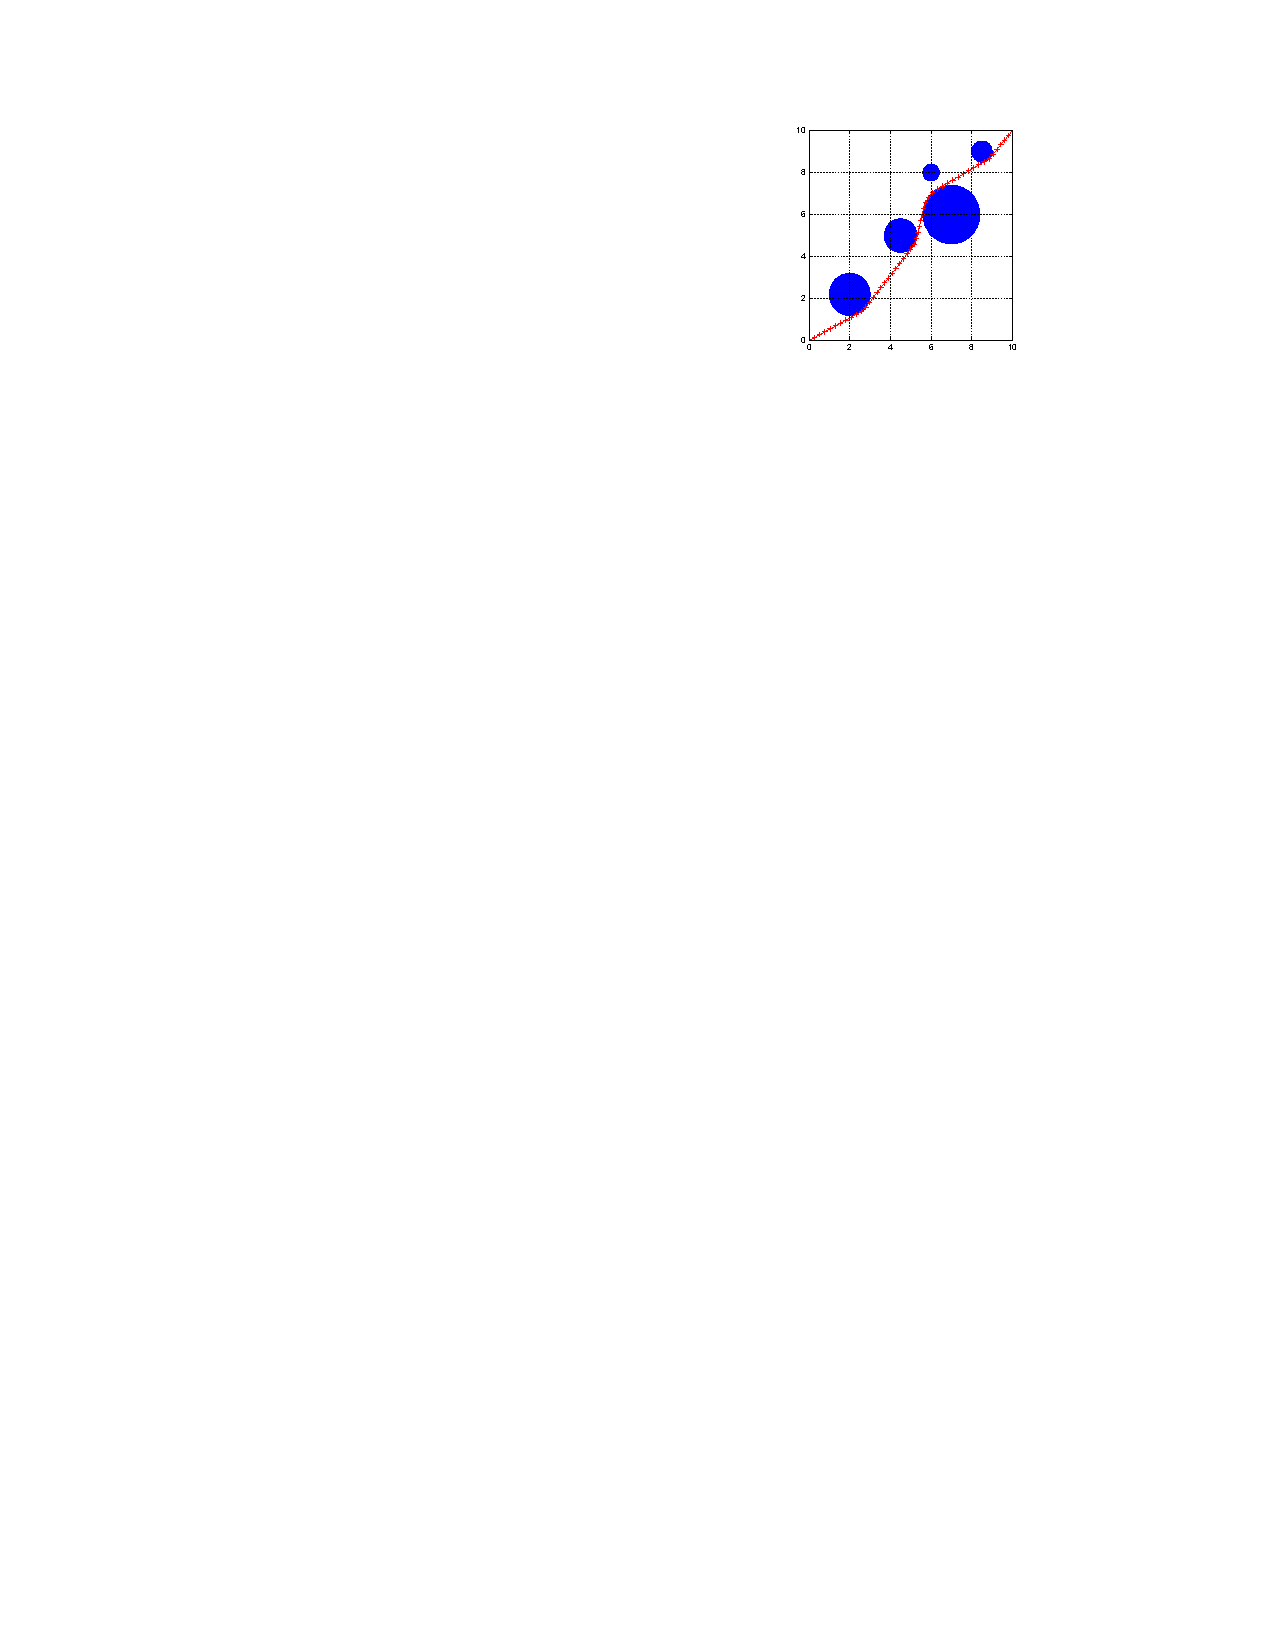
\includegraphics[width=0.4\textwidth]{path_planning.pdf}
\end{center}
\end{frame}

\begin{frame}{Floor planning}
\BIT
\item $n$ rectangles with lower left corner $(x_i, y_i)$, $i=1,\ldots, n$ (variables)
\item rectangle $i$ has width $w_i$, height $h_i$ (given)
\item centers are $c_i = (x_i+w_i/2, y_i + h_i/2)$
%\item all rectangles lie inside bounding rectangle with given width $W$ and height $H$
%\[
%0 \leq x_i, \quad 0 \leq y_i, 
%\quad x_i + w_i \leq W, \quad
%y_i + h_i \leq H, \quad i=1, \ldots, n
%\]
\item edge set $\mathcal{E} \subset \{1,\ldots, n\}^2$ 
contains pairs of rectangles we want to be close
\item minimize $\sum_{(i,j)\in \mathcal E} \|c_i - c_j\|_2^2$
\item without loss of generality, we can require
$(1/n)\sum_{i=1}^{n} c_i = 0$
\item these constraints and objective are convex; non-overlapping constraint is not
\EIT
\end{frame}

\begin{frame}{Non-overlapping constraint}
\BIT
\item rectangles $i$ and $j$ don't overlap if
\[
x_i + w_i \leq x_j \quad \lor \quad x_j + w_j \leq x_i \quad \lor \quad
y_i + h_i \leq y_j \quad \lor \quad y_j + h_j \leq y_i, \quad i < j
\]
\ie, rectangle $i$ is left of, right of, below, or above rectangle $j$
\item express as inequality
\[
\min \left(x_i+w_i-x_j, x_j+w_j-x_i, y_i+h_i-y_j, y_j+h_j-y_i\right) \leq 0
\]
\item left-hand side is concave function of $(x,y)$
\item so non-overlapping can be expressed as a DC inequality constraint
\EIT
\end{frame}

\begin{frame}{Floor planning as DC problem}
\BIT
\item DC formulation of floor planning problem:
\[
\begin{array}{ll}
\mbox{minimize}
& \sum_{(i, j) \in \mathcal{E}} \|c_i - c_j\|_2^2\\
\mbox{subject to}
& \sum_{i=1}^n c_i = 0, \quad c_i = (x_i+w_i/2, y_i + h_i/2), \quad i = 1,\ldots, n,\\
& \min \left(x_i+w_i-x_j, x_j+w_j-x_i, y_i+h_i-y_j, y_j+h_j-y_i\right) \leq 0, \quad i < j
%& 0 \leq x_i \leq W - w_i, \quad 0 \leq y_i \leq H - h_i, \quad i = 1,\ldots, n,
\end{array}
\]
\item $x_i$, $y_i$, and $c_i$ are variables;
$w_i$, $h_i$, and $\mathcal{E}$ are given
\EIT
\end{frame}

\begin{frame}{Floor planning example}
$n=6$ rectangles; initial centers drawn uniformly from $[-2, 2]^2$
\vfill
\centering
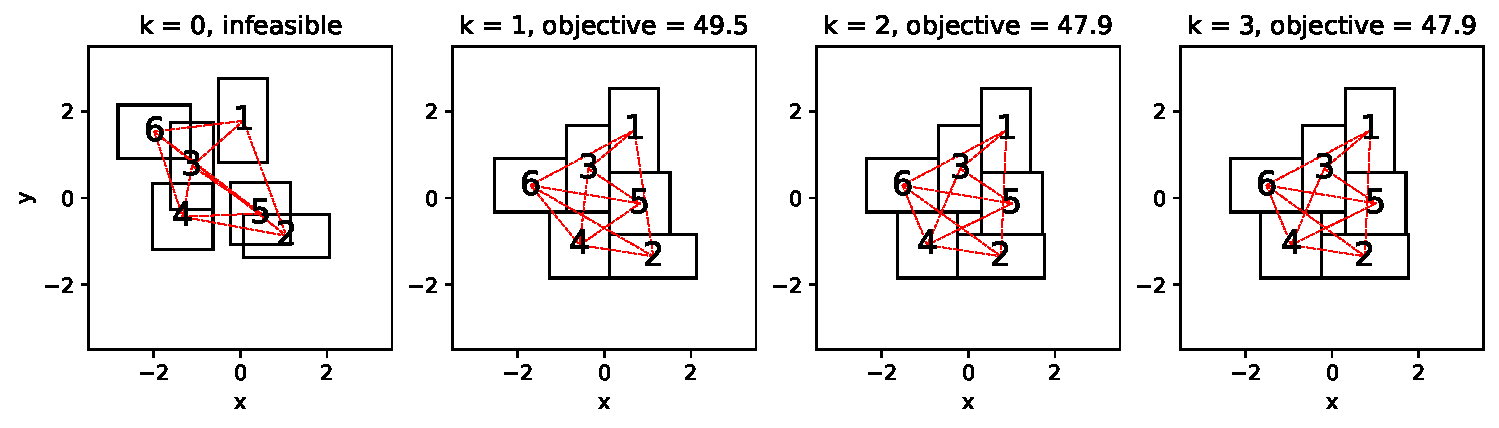
\includegraphics[width=\textwidth]{floor_planning_seed23.pdf}
\end{frame}

\begin{frame}{Floor planning example}
\centering
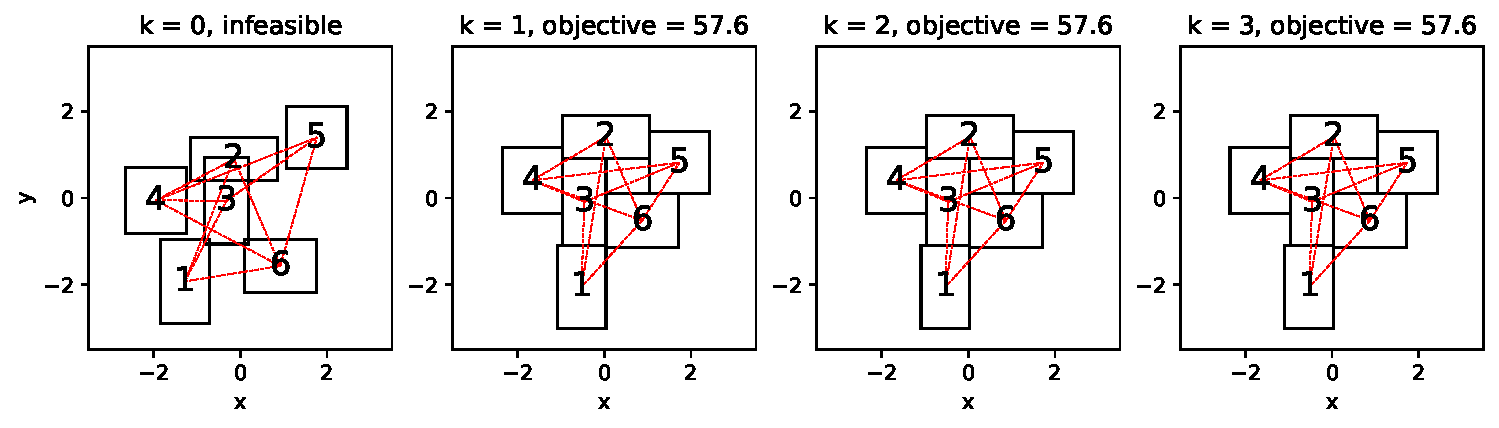
\includegraphics[width=\textwidth]{floor_planning_seed11.pdf}
\end{frame}

\begin{frame}{Floor planning example}
\centering
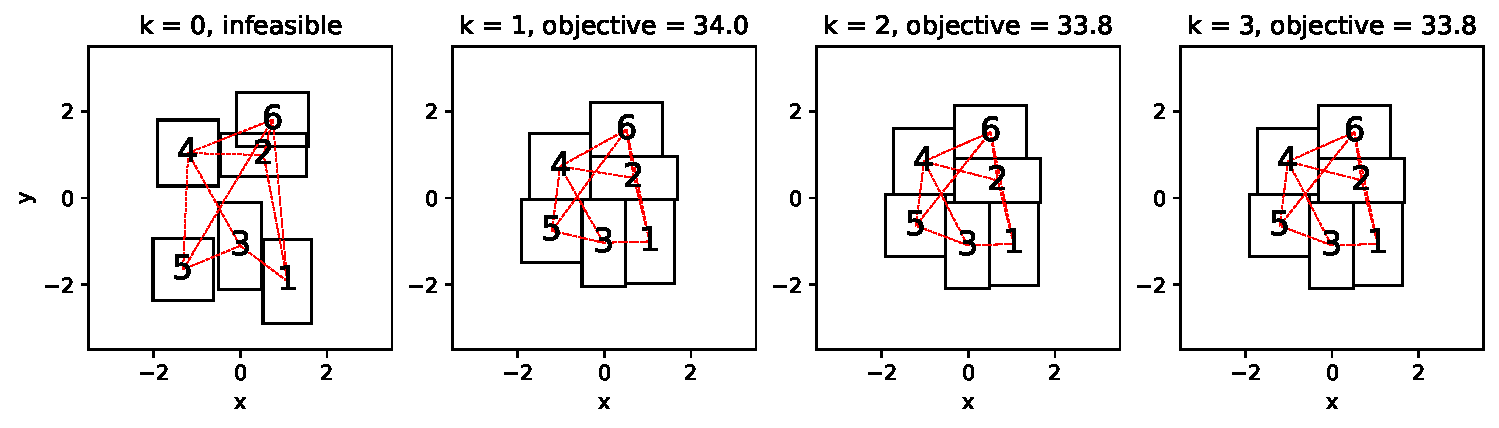
\includegraphics[width=\textwidth]{floor_planning_seed10.pdf}
\end{frame}

\begin{frame}{Floor planning example}
\centering
% 100 trials, value after 5 iterations
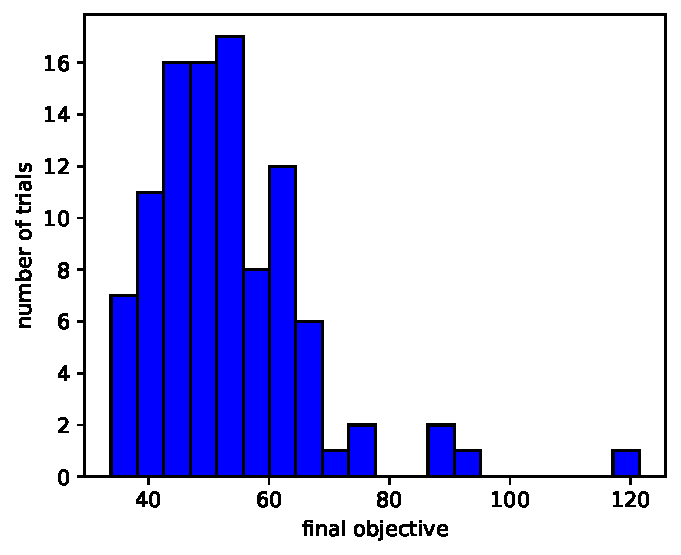
\includegraphics[width=0.5\textwidth]{floor_planning_hist.pdf}
% can compute lower bound as sum of min((w_i + w_j)/ 2, (h_i + h_j)/2)
% taking the sqrt, we get roughly 4
% sqrt of minimal objective among 100 is about 6
\end{frame}

\begin{frame}{Collision avoidance}
\BIT 
\item $N$ vehicles moving simultaneously along (discretized) time $t = 0, \ldots, T$
\item vehicle $i$ aims to travel from initial position $x_i^\text{init}$
to final position $x_i^\text{final}$
\item trajectories described as
\[
x_{i,t}, \quad i = 1, \ldots, N, \quad t = 0, \ldots, T
\]
\item vehicles must keep minimum distance $d$ from each other at all times
\EIT
\end{frame}

\begin{frame}{Collision avoidance}
\BIT
\item minimize total length of travel while avoiding collisions as
\[
\begin{array}{ll}
\mbox{minimize} & \sum_{i=1}^{N} L_i\\
\mbox{subject to} & x_{i, 0} = x_i^\text{init}, \quad x_{i, T} = x_i^\text{final},
\quad i = 1, \ldots, N, \\
& \|x_{i, t} - x_{i, t-1}\|_2 \leq L_i/T, \quad i = 1, \ldots, N, \quad t = 1, \ldots, T, \\
& \|x_{i, t} - x_{j, t}\|_2 \geq d, \quad i < j, \quad t = 0, \ldots, T
\end{array}
\]
\item $x_{i,j}$ and $L_i$ are variables
\item  $x_i^\text{init}$,  $x_i^\text{final}$, and $d$ are given
\EIT
\end{frame}

\begin{frame}{Collision avoidance example}
\begin{columns}
\begin{column}{0.7\textwidth}
\BIT
\item $N = 10$ vehicles with starting points $x^\text{init}_i$ uniformly on a circle around zero
\item each vehicle aims to travel to opposite side of circle, $x^\text{final}_i = -x^\text{init}_i$
\item minimum distance is $d=1$
\EIT
\end{column}
\begin{column}{0.3\textwidth}
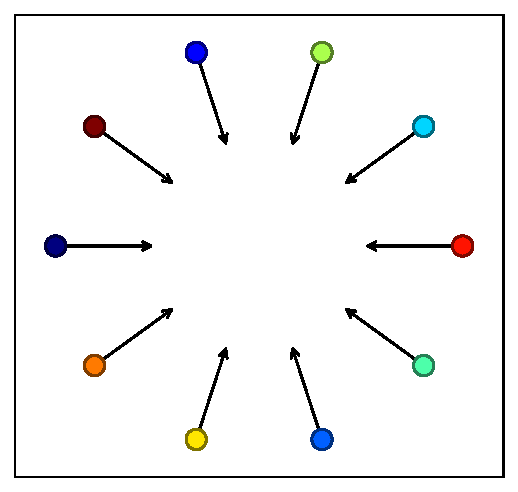
\includegraphics[width=\textwidth]{collision_avoidance_setting.pdf}
\end{column}
\end{columns}
\end{frame}

\begin{frame}{Collision avoidance example}
\centering
%\animategraphics[loop,autoplay,width=0.5\textwidth]{25}{collision_avoidance_frame}{1}{74}
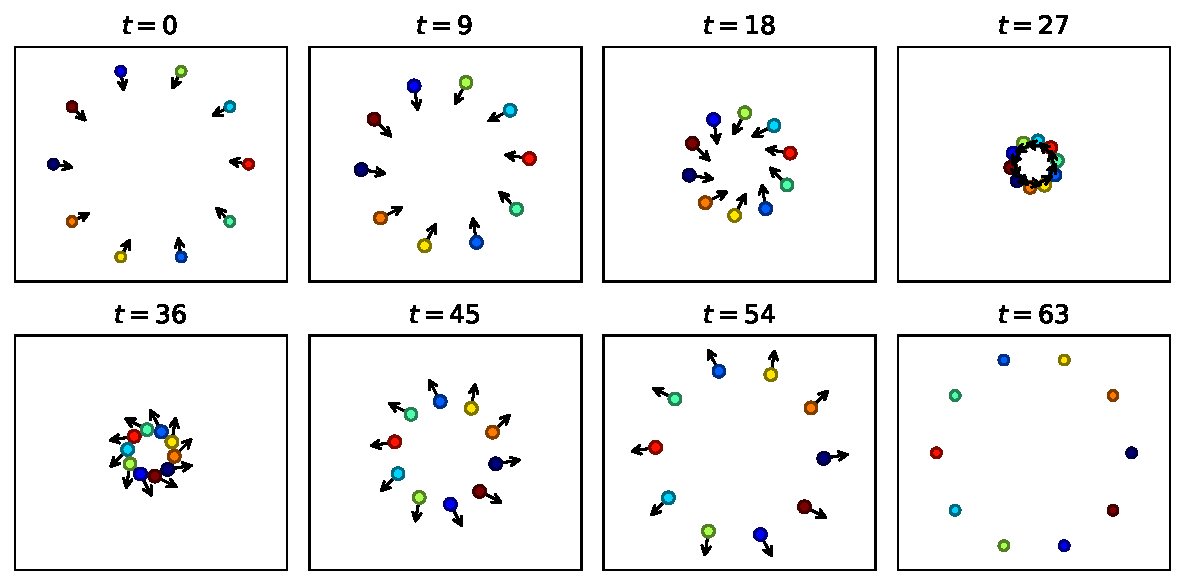
\includegraphics[width=\textwidth]{collision_avoidance_frames.pdf}
\end{frame}

\iffalse
\begin{frame}{Sphere embedding}
\BIT
\item want to embed $N$ points $x_1, \ldots, x_N$ on the sphere $\{x \in \reals^n \mid \|x\|_2 = 1\}$
\item set $\mathcal{C} \subset \{1, \ldots, N\}^2$ contains pairs of points we want to be close
\item set $\mathcal{F} \subset \{1, \ldots, N\}^2$ contains pairs of points we want to be far apart
\item minimize $\sum_{(i, j) \in \mathcal{C}} \|x_i - x_j\|_2^2 - \sum_{(i, j) \in \mathcal{F}} \|x_i - x_j\|_2^2$
\item quadratic DC function where PSD and NSD parts are already separated
\item can write sphere containment as
\[
\|x_i\|_2 \leq 1, \quad \|x_i\|_2 \geq 1, \quad i = 1, \ldots, N
\]
first constraint is convex, second constraint is concave
\EIT
\end{frame}

\begin{frame}{Sphere embedding}
\BIT
\item solve
\[
\begin{array}{ll}
\mbox{minimize} & \sum_{(i, j) \in \mathcal{C}} \|x_i - x_j\|_2^2 - \sum_{(i, j) \in \mathcal{F}} \|x_i - x_j\|_2^2\\
\mbox{subject to} & \|x_i\|_2 \leq 1, \quad \|x_i\|_2 \geq 1, \quad i = 1, \ldots, N
\end{array}
\]
\item $x_i$ are variables
\item $\mathcal{C}$ and $\mathcal{F}$ are given
\EIT
\end{frame}

\begin{frame}{Sphere embedding example}
\BIT
\item \textbf{example:} embedding $N=\ldots$ points in $n=3$ dimensions
\EIT
\end{frame}
\fi

\begin{frame}{$\ell_{1/2}$ regularized regression}
\BIT
\item minimizing $\|Ax-b\|_2^2+\lambda \| x\|_1$ where $A \in \reals^{m \times n}$ tends to yield \textbf{sparse} $x$
\item (approximately) 
minimizing $\|Ax-b\|_2^2+\lambda \sum_i |x_i|^{1/2}$ can yield \textbf{sparser} $x$
\item sometimes called $\ell_{1/2}$ regularization (but it's not a norm)
\item not a convex problem
\EIT
\end{frame}

\begin{frame}{DC formulation}
\BIT
\item DC problem
\[
\begin{array}{ll} \mbox{minimize} & \|Ax-b\|_2^2 + \lambda \ones^T t\\
\mbox{subject to} & t \succeq 0, \quad |x_i| \leq t_i^2, \quad i=1,\ldots, n
\end{array}
\]
\item CCP: $x^{k+1}$ is solution of
\[
\begin{array}{ll} \mbox{minimize} & \|Ax-b\|_2^2 + \lambda \ones^Tt\\
\mbox{subject to} & t \succeq 0, \quad |x_i| \leq 
(t^k_i)^2+2t_i^k(t_i-t_i^k),\quad i=1,\ldots, n
\end{array}
\]
\item so $x^{k+1}$ is solution of weighted $\ell_1$ regularized problem
\[
\begin{array}{ll} \mbox{minimize} & \|Ax-b\|_2^2
 +\lambda \sum_{i=1}^n \frac{1}{2t_i^k} |x_i|
\end{array}
\]
with $t_i^{k+1}= \frac{1}{2t_i^k}|x_i^{k+1}| + \frac{1}{2}t_i^k$
(we can impose a small minimum value for $t_i^{k}$)
\EIT
\end{frame}

\begin{frame}{Example}
\BIT
\item example with $n = 20$, $m = 40$
\item regularization paths for $\ell_1$ (left) and $\ell_{1/2}$ (right) regularization 
\EIT

\vfill

\begin{columns}
\begin{column}{0.5\textwidth}
\centering
%$\ell_1$ regularization \\
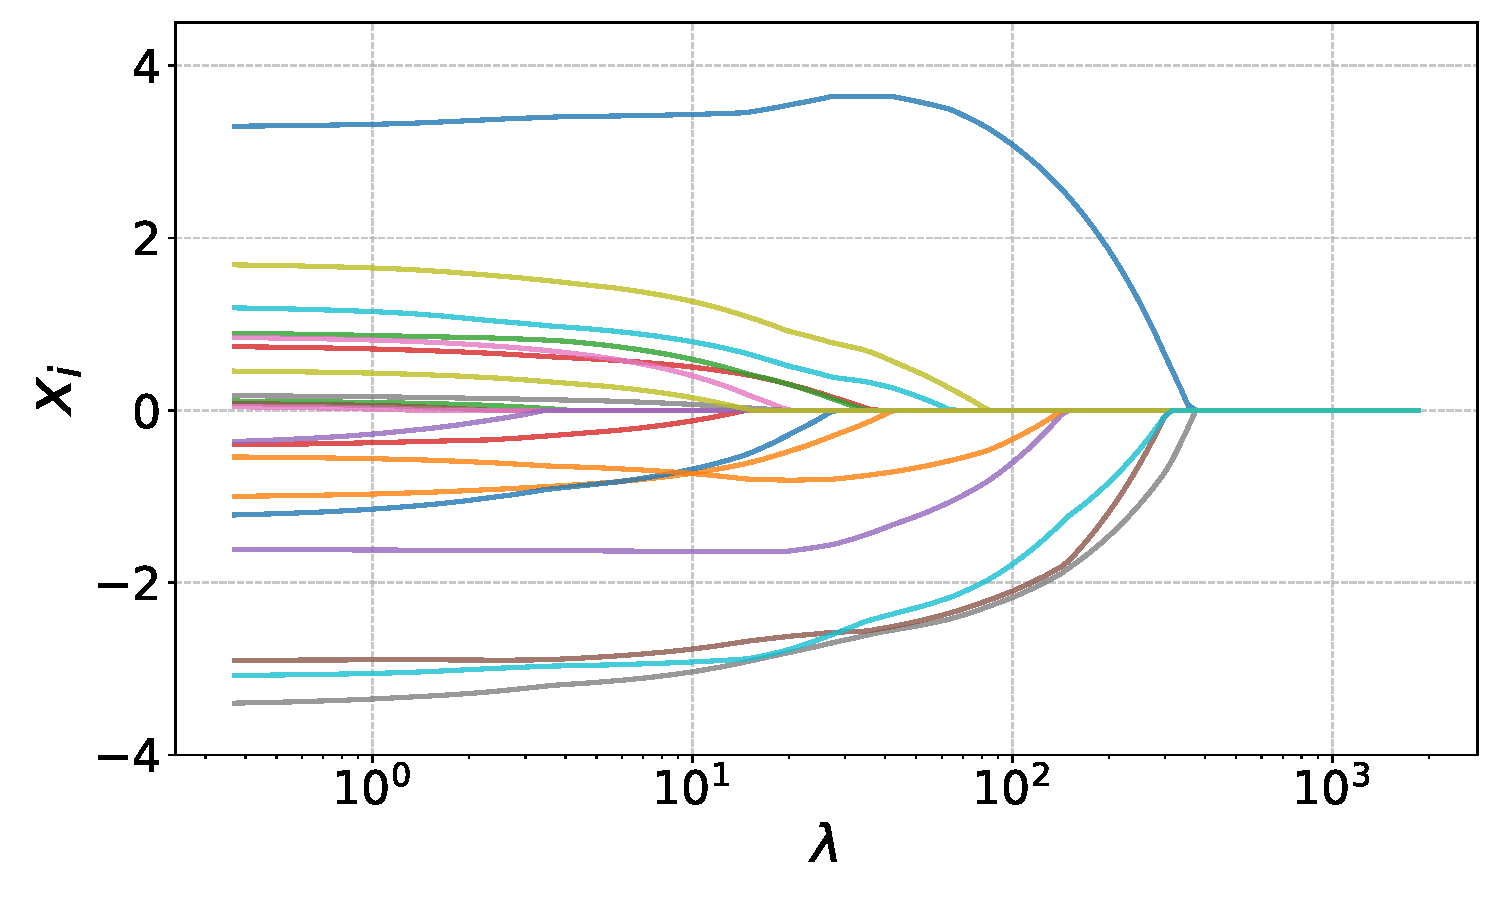
\includegraphics[width=\textwidth]{lasso_reg_path_larger.pdf}
\end{column}
\begin{column}{0.5\textwidth}
\centering
%$\ell_{1/2}$ regularization \\
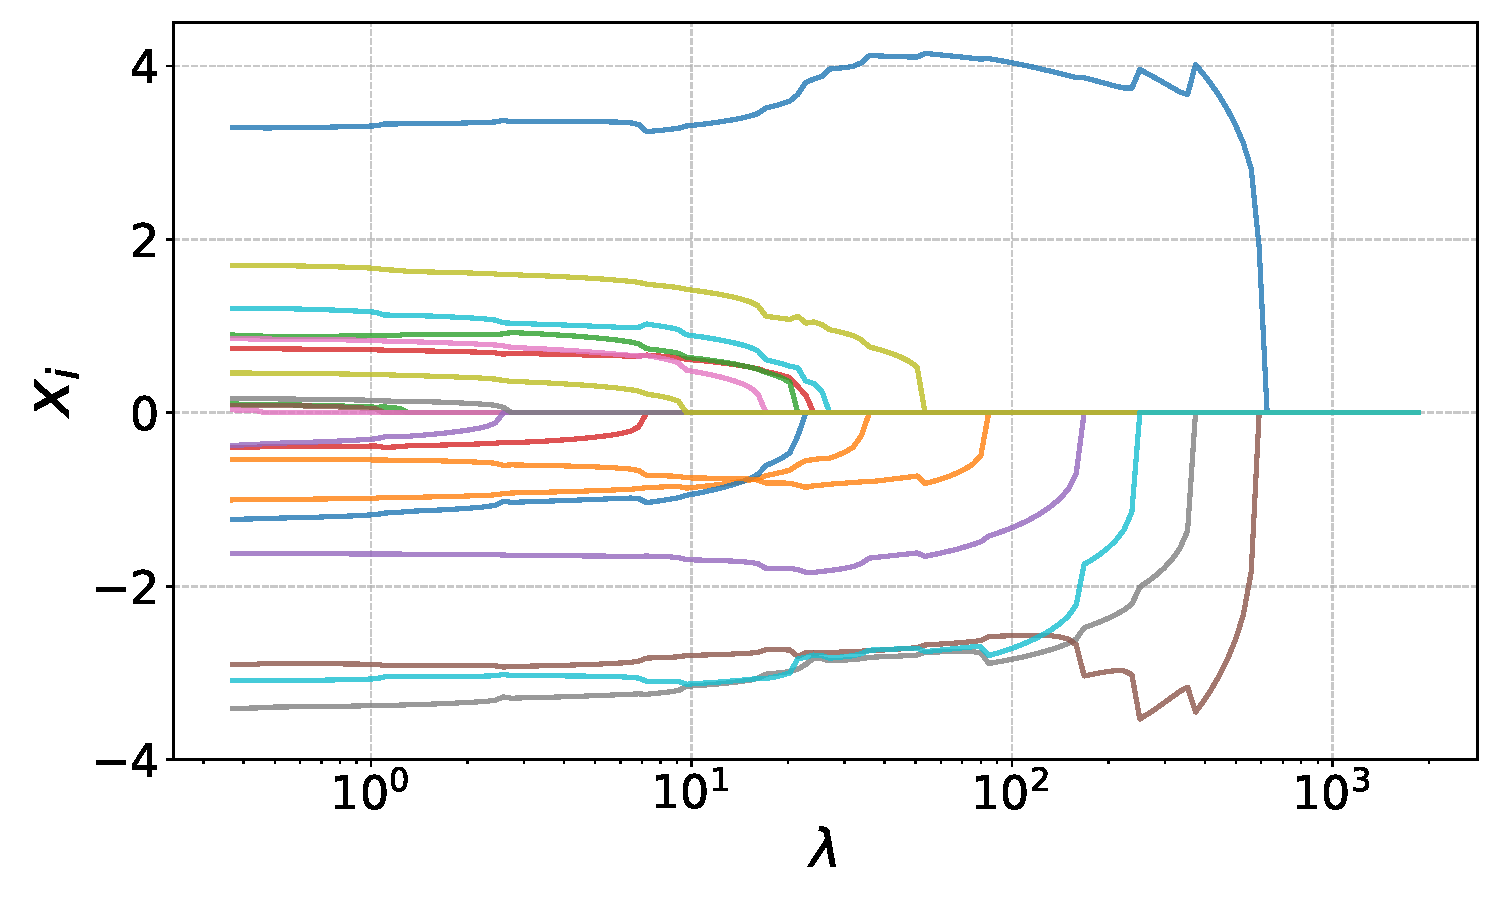
\includegraphics[width=\textwidth]{ell_half_reg_path_larger.pdf}
\end{column}
\end{columns}
\vfill\centering
\end{frame}

\begin{frame}{Example}
\centering
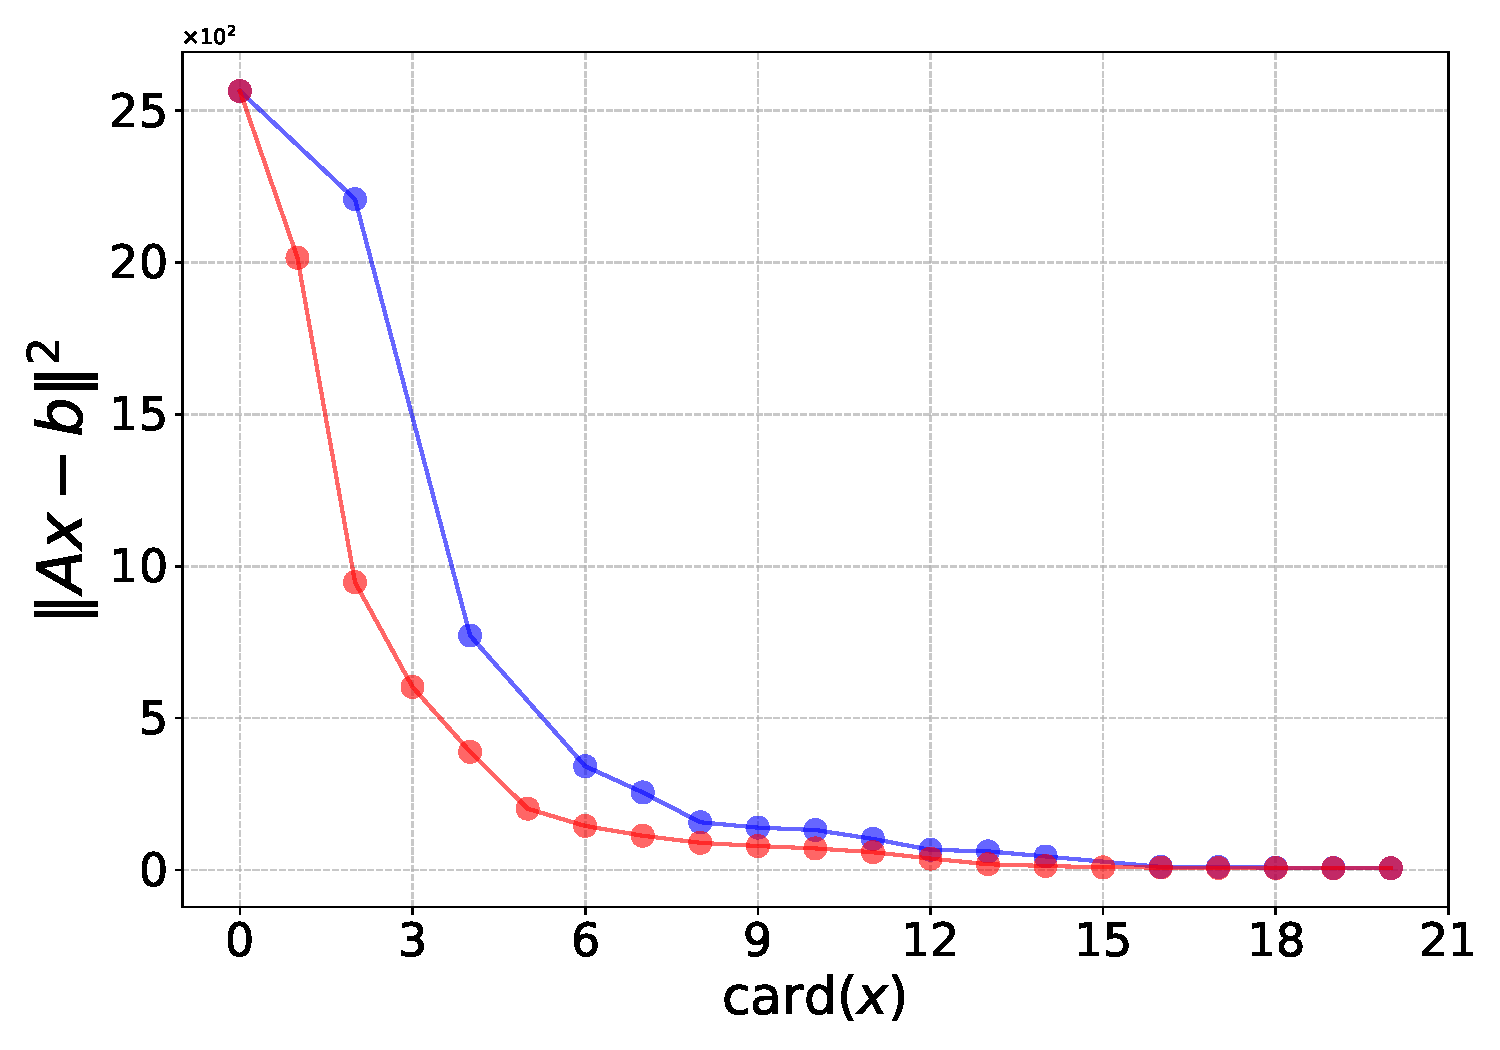
\includegraphics[width=0.60\textwidth]{pareto_curve_version2.pdf}
\vfill\centering

optimal trade off curves for $\ell_1$ (\textcolor{blue}{blue}) and 
$\ell_{1/2}$ (\textcolor{red}{red}) regularization
\end{frame}

%\begin{frame}{Example}
%\centering
%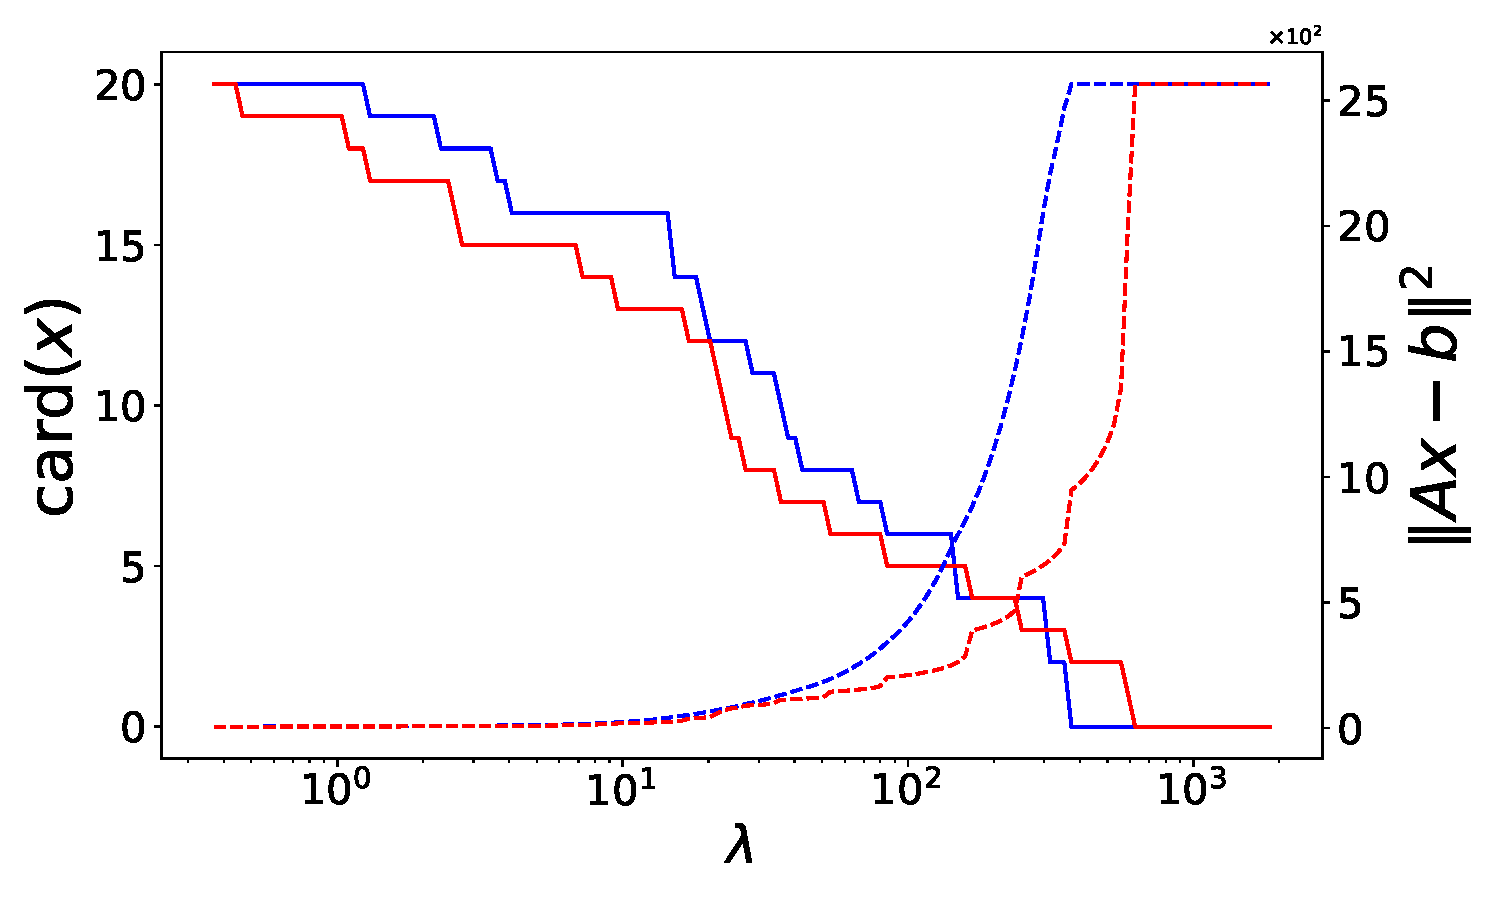
\includegraphics[width=0.70\textwidth]{card_and_fit.pdf}
%
%cardinality and fit versus regularization for $\ell_1$ (\textcolor{blue}{blue}) and $\ell_{1/2}$ (\textcolor{red}{red}) regularization
%\end{frame}

\iffalse
\begin{frame}{Regressor selection}
\BIT
\item norm approximation problem: choose $x$ to minimize $\|Ax-b\|_2$
\item optimal $x$ is $A^\dagger b$; optimal error is $ \|A A^\dagger b-b\|_2$
\item regressor selection: find sparsest $x$ subject to 
$\|Ax-b\|_2 \leq \kappa$, with $\kappa > \|A A^\dagger b-b\|_2$ 
\[
\begin{array}{ll}
\mbox{minimize} & \mathbf{card}(x) \\
\mbox{subject to} & \|Ax-b\|_2 \leq \kappa
\end{array}
\]
with variable $x$;
$\mathbf{card}(x)$ is number of nonzero entries (cardinality) of $x$
\EIT
\end{frame}

\begin{frame}{Regressor selection}
\BIT
\item DC formulation:
\[
\begin{array}{ll}
\mbox{minimize} & \ones^T q \\
\mbox{subject to} & |x_i| \leq M q_i, \quad 0 \leq q_i \leq 1,
\quad q_i - q_i^2 \leq 0, \quad i = 1, \ldots, n, \\
& \|Ax-b\|_2 \leq \eta \|A A^\dagger b-b\|_2,
\end{array}
\]
with variables $x \in \reals^n$, $q \in \reals^n$ 
\item $M > 0$ is chosen to be sufficiently large
\item called \textbf{big-$M$ method}
\EIT
\end{frame}
\fi

\end{document}
